\documentclass{article}
\usepackage[utf8]{inputenc}
\usepackage{graphicx}
\usepackage{listings}  
\title{Fight Mosquitoes with Mosquitoes}
\author{Aditi Kabra, Divyansh Garg, Dang Pham}
\date{November 2016}

\begin{document}

\maketitle

\tableofcontents

\vspace{15cm}

\section{Introduction and Problem Statement}

The Zika virus is currently a major global health concern. Capable of mosquito-human transmission, the Zika epidemic can easily and rapidly spread through almost-omnipresent mosquitoes. If a pregnant woman has Zika, her child may be born with serious birth defects. Although Zika is capable of high distribution power and no cure nor vaccine has been found targeting the vector of the disease - the mosquito - will be an effective best solution. Thus, there are three possible way to neutralize the epidemic:
\begin{enumerate}
    \item Human behavioral measures (long-sleeved shirts, insects repllant, etc).
    \item Reducing the local mosquito population.
    \item Reducing mosquitoes' capability to transmit Zika.
\end{enumerate}

(2) and (3) can be accomplished by introducing "modified mosquitoes". These mosquitoes carry \textit{Wolbachia bacterium}. Female \textit{Wolbachia} are far less likely to carry Zika and male \textit{Wolbachia} will not produce offspring with normal mosquitoes. The table in Section 3.2 will further detail the interactions between mosquitoes.\\

This paper's goal is determine the minimum number of male \textit{Wolbachia} and the number of female \textit{Wolbachia} to be released every month for 5 years to control the number of mosquitoes capable of transmitting Zika. \\ 

The parameters our model will ensure (as the prompt requires) are:
\begin{itemize}
    \item The total number of pregnant women infected within 5 years will not exceed 10,000.
    \item After the first year, no more than 300 people are newly infected per day.
\end{itemize}

Our team has two approaches to the problem: a deterministic mathematical model (in Section 3) and a computer simulation (in Section 4) to check the result from the math model. Using both, we can have an accurate depiction of the problem and a possible, realistic solution to employ to eliminate the epidemic. In section 2, we have made a series of assumption. Most are from the prompt and from data to be found in past research. A few we have had to make to the best of our own ability due to lack of data. Finally, we will discuss the solution, implementation, strengths and weaknesses, and future work to be accomplished. 

\section{Model Assumptions}
\textbf{A.} The following assumptions made from the data given by the prompt: 
\begin{enumerate}
    \item \textit{Wolbachia}-infected mosquitoes cannot become Zika-infected.
    \item 1\% of initial mosquitoes population has Zika. 
    \item Initially, 22 pregnant women get newly Zika-infected. 
    \item Initially, 600 new people are infected per day.
\end{enumerate}

Based on experimented data collected from past research, we are able to collect vital assumptions to help us closely model the real world. We use these as initial conditions and constraints for the models listed below. It is necessary to have these to break the possible degeneracy so as to accurately determine the solutions and align them to realistic implementation.\\ \\
\textbf{B.} The following data-driven assumptions are made: 
\begin{enumerate}
    \item Normal mosquitoes are assumed to be of genus \textit{Aedes}. Since Zika disease vectors are mainly \textit{Aedes} genus mosquitoes (Center for Disease Control), we will assume normal mosquitoes to be \textit{Aedes}. Furthermore, data below related to mosquito development, lifespan, etc. are primarily from this genus. 
    \item The gender ratio of mosquitoes is 1:1 (Lounibos \& Escher, and Mayer). This assumption is also logical as nature would tend to stabilize the population at equilibrium.
    \item Only female mosquitoes bite human (National Geographic). Thus, they will the focus of our modeling.
    \item A female mosquitoes will lay approximately 100 eggs in one hatching (Center for Disease Control).
    \item Typically, only 1 to 10 percent of eggs become adult mosquitoes (Beck-Johnson et. al).
    \item It takes around 7-10 days for the eggs to become adult mosquitoes (Center for Disease Control). 
    \item Average temperature of Puerto Rico is about 80$^{\circ}$F or 27$^{\circ}$C (National Weather Service).
    \item Mosquitoes and its larvae optimal condition for growth and living is 27$^{\circ}$C (Beck-Johnson et. al), coinciding to that of Puerto Rico. In this condition, we the assume male mosquitoes to live about 7-10 days (Illinois Department of Public Health), and female to last 2-3 weeks (Beck-Johnson et. al).
    \item Although female mosquitoes can transmit Zika to her offspring and eggs, we deem the chances (1 in 290) to be negligible (Thangamani et al.). This female-offspring transmission will keep existence of Zika in the population in the long term (Thangamani et al.). However, since the scope of this paper is short-term (5 years) this effect is negligible.
    \item Because of assumption (B9), the only way a new mosquito can become Zika-infected is if it bites a Zika-infected human. 
    \item The Zika virus stays in a human for two weeks. The human immunity eliminates the virus after this time period - the human is no longer infectious (Johnson - StatNews).
    \item Due to lack of data on Zika immunity, we assume if a person is Zika-infected, then cleared of Zika two weeks later, but then gets bitten by a Zika-infected mosquito, the person can still re-attain Zika. This assumption is made for the worst case scenario, which the model has to take into consideration to assure the predicted results.
    \item Following the assumption made by \textit{Beck-Johnson et al.}, we assume a constant adult mosquito mortality rate of 10\% per day.
    \item Puerto Rico population is 3.5 million, and as of July 2016, 5000 cases have been diagnosed (NPR,CDC). Assuming that 80\% of cases are undiagnosed and using a progression from July to the current time (November), we estimate that currently there are 25,000 people with Zika.
    \item The average mosquito density per house in Puerto Rico ranges from 5-30 (Chaves and Morrison) - averaging 17.5 mosquitoes per households.
    \item There are about 1.3 million households in Puerto Rico (U.S. 2010 Census) where each house has 2.68 people.
    \item From (B15) and (B16) there is an average of 22.75 million mosquitoes in Puerto Rico.
    \item From assumption B15 and B14, we know that there are 17.5 mosquitoes in a household with 2.68 people. The biting rate will be $\frac{2.68}{17.58}\approx0.15$.
\end{enumerate}

\textbf{C.} We also make the following trivial assumptions:
\begin{enumerate}
    \item We assume released \textit{Wolbachia} mosquitoes are newly hatched.
    \item We assume that a male mosquito is Wolbachia or regular does not influence its chance of fertilizing an egg.
    \item We will assume that the total population stays constant as people do not die from Zika and babies are not old enough to have more babies in 5 years.
    \item We will ignore the incubation period of Zika (it comes in to effect instantly).
    \item We will assume that the transmission rate from mosquitoes to human is 100\% (i.e. if the mosquito bite a Zika-infected human, it certainly gets Zika)
\end{enumerate}

\section{Deterministic Mathematical Model}
\subsection{Notation}
The following notation will be used for simplification:
\begin{itemize}
    \item W are \textit{Wolbachia} mosquitoes.
    \item R are regular mosquitoes.
    \item $N_R$ and $N_W$ are total number regular mosquitoes and \textit{Wolbachia} mosquitoes respectively.
    \item Null means no mosquitoes exist.
    \item $\alpha$ is the birth rate.
    \item $\gamma$ is the mortality rate.
    \item $M_W$ and $F_W$ are male and female \textit{Wolbachia} respectively.
    \item $M_R$ and $F_R$ are male and female regular mosquitoes respectively.
    \item $N_z$ is the number of Zika-infected females mosquitoes (only female mosquitoes bite from assumption B3 and the only way Zika is transmitted to mosquitoes is through biting from assumption B9, thus, all the number of Zika-infected mosquitoes are females).
    \item $N_h$ is the number of Zika-infected humans.
    \item $H$ is the total human population.
    \item $F_R$ is the number of female regular mosquitoes (again since male mosquitoes do not bite, we can neglect them).
    \item $k$ is the number of human bitten per mosquito per day (biting rate of mosquito per day).
    \item $p_1$ is the probability of zika transmission from human to mosquito.
    \item $p_2$ is the probability of zika transmission from mosquito to human.
    \item $D_h$ is the duration of Zika virus in the human body (from B11, so $D_h=14$ days)
    \item Subscript $_0$ indicates initial (e.g. $M_{W0}$ means the initial male \textit{Wolbachia}
    population.
    \item $N_t$ is the total number of humans infected.
 \end{itemize}
\subsection{Population Dynamics with \textit{Wolbachia}}

Following the prompt, we can easily arrive at the following table detailing the interaction between \textit{Wolbachia} mosquitoes and regular mosquitoes (without Zika - Zika mosquitoes will be accounted later).
\begin{center}
\begin{tabular}{ c| c c}
       & M_R$  & $M_W$ \\ 
       \hline
 $F_R$ & R & Null \\  
 $F_W$ & W & W    
\end{tabular}
\end{center}

For regular mosquitoes, the birth rate is dependent on the number of female $F_R$ and the birth factor $\alpha$ assumed to be a constant.
We do not consider dependency on $M_R$ because there is no limit on the number of eggs a male mosquito might fertilize. 
The birthrate is also proportional to the percentage of male \textit{Wolbachia} over total males, $\frac{M_R}{M_R + M_W}$. Thus, it is equal to $\frac{\alpha F_R M_R}{M_R + M_W}. \\

For the mortality rate $\gamma$, it is assumed to be linearly dependent on $N_R = M_R + F_R$, i.e. the number of mosquitoes death per day is constant (following assumption B13). Using the result from $\alpha$ and $\gamma$, we can then write the equation relating the change of total population $N_R$ of regular mosquitoes over time. 
\begin{equation}
    \frac{dN_R}{dt}= \frac{\alpha F_R M_R}{M_R+M_W} - \gamma N_R
\end{equation}

Using assumption B2, the sex ratio is 1:1,therefore $F_R = M_R = \frac{N_R}{2}$.\\

Initially at $t=0$, without any \textit{Wolbachia} mosquitoes, the population is at steady state, so:
\begin{center}
    $\alpha F_R = \gamma N_R = 2 \gamma F_R \rightarrow \alpha = 2\gamma$
\end{center}

Following a similar approach to equation 1 to find the rate for male \textit{Wolbachia} we find that:
\begin{equation}
    \frac{dM_W}{dt} = \frac{\alpha}{2} F_W - \gamma M_W
\end{equation}
Note that the $\frac{\alpha}{2}$ factor exists because we are assuming 50\% of offspring are male. Then similarly, for female \textit{Wolbachia} mosquitoes we find that: 
\begin{equation}
    \frac{dF_W}{dt} = \frac{\alpha}{2} F_W - \gamma F_W
\end{equation}

We can assume that the mortality and birth rate of \textit{Wolbachia} mosquitoes to be the same as that of regular mosquitoes. Now for equation (3) as $\alpha = 2\gamma$, we have $\frac{dF_w}{dt} = 0 \rightarrow F_W = F_{W0} $.\\

Substituting the result into equation (2), we have:
\begin{center}
$\frac{dM_w}{dt} = \frac{\alpha}{2} F_{W0} - \gamma M_W$\\ $\\
$\rightarrow M_W = F_{W0} + (M_{W0} - F_{W0})e^{-\gamma t}$\\
\end{center}

Now we can further simplify equation (1) with a 1:1 sex ratio to:
\begin{center}

$\frac{dF_r}{dt} = \frac{\alpha}{2}\frac{F_R^2}{F_R+M_W}-\gamma F_R$
\end{center}

With $\alpha = 2\gamma$ as derived before:
\begin{equation}
    \frac{dF_R}{dt} = -\frac{\gamma F_R M_W}{F_R + M_W}
\end{equation}

This equation (4) along with $M_W = F_{W0} + (M_{W0} - F_{W0})e^{-\gamma t}$ govern the population dynamics of mosquitoes.
\subsection{Mosquitoes-Human Interaction}

Using assumptions (C3) and (C4), we know that the number of $F_R$ infected per day depends only on the number of humans bitten per mosquito per day, the probability of transmission human to mosquito, the fraction of infected human population and the number of non-infected $F_R$.
Also including the death rate of the mosquitoes, we can write:
\begin{equation}
    \frac{dN_z}{dt} = kp_1\frac{N_h}{H}(F_R - N_z) - \gamma N_z
\end{equation}

Similarly, the number of humans infected per day depends on the number of humans bitten per mosquito per day, the probability of transmission from mosquito to human, the fraction of non-infected humans and the number of infected mosquitoes. Also, from assumption B11, the Zika virus only stays in the body for 2 weeks, hence we approximate the number of humans cured per day as the number of humans infected divided by the duration of infection (2 weeks = 14 days).\footnote{This is a reasonable approximation because around $1/14^{th}$ of the people currently infected had been infected fourteen days ago. This is true since there is no extremely sharp spike or drop in the number of people infected.} Thus, we have:

\begin{equation}
    \frac{dN_h}{dt} = kp_2N_z (\frac{H-N_h}{H}) - \frac{N_h}{D_h}
\end{equation}
where $D_h=14$ days. Using equation (5), (6), and $F_R$ estimated using the population dynamics model, we can model the infection transmission interaction between humans and mosquitoes.
\subsection{Total Number of Humans Infected}
The total number of humans infected is a simple modification of equation (6). We need to remove the curing factor since we want the total amount of infected people. Thus, equation (6) becomes:
\begin{equation}
    \frac{dN_t}{dt} = kp_2N_z (\frac{H-N_h}{H})
\end{equation}

However, this simple approach creates a problem of over-counting. That is,  $N_t(t)$ counts a person 14 times more (contrasting to when the person was cured - refer to footnote 1). To counter this, we need to divide the total by $D_h=14$. However, our model is numerically able to predict this correction factor, which differs a bit from 14 since our model is not perfect in the sense that it does not account for a delay in mosquito birthing rate (read more in strengths and weaknesses and future works). \\

For now, we will call this factor $\epsilon$. $\epsilon$ will be addressed and derived in the Model Results section. For now, the equation governing the total number of Zika-infected is then:
\begin{equation}
    \frac{dN_t}{dt} = \frac{1}{\epsilon}kp_2N_z (\frac{H-N_t}{H})
\end{equation}

\subsection{Initial Conditions and Constants}
We will re-condense the equations from previous sections to here for brevity and easy referencing.\\

We need to solve the following system of equations.
\begin{equation}
    \frac{dF_R}{dt} = -\frac{\gamma F_R M_W}{F_R + M_W}
\end{equation}
\begin{equation}
    \frac{dN_z}{dt} = kp_1\frac{N_h}{H}(F_R - N_z) - \gamma N_z
\end{equation}
\begin{equation}
    \frac{dN_h}{dt} = kp_2N_z (\frac{H-N_h}{H}) - \frac{N_h}{D_h}
\end{equation}
where
\begin{equation}
    M_W = F_{W0} + (M_{W0} - F_{W0})e^{-\gamma t}
\end{equation}
in order to find $N_h$, which allows us to know how many people are infected at a certain time.\\

In addition, to model the mosquitoes population dynamics we need to solve the following equations:
\begin{equation}
    \frac{dF_w}{dt} = (\frac{\alpha}{2}F_w)-\gamma F_w
\end{equation}
\begin{equation}
    \frac{dM_w}{dt} = (\frac{\alpha}{2}F_w)-\gamma M_w
\end{equation}
\begin{equation}
    \frac{dN_t}{dt} = \frac{1}{\epsilon}kp_2N_z (\frac{H-N_t}{H})
\end{equation}

Our final goal is to solve for $N_t(1825)$ to find the total of Zika-infected humans after 5 years (1825 days). Now we need to get the constants and initial conditions from data and assumptions:
\subsubsection{Constants}
\begin{enumerate}
    \item $\gamma$ = 10\% per day or 0.1 (assumption B13).
    \item $\alpha = 2\gamma = 0.2$  (from Section 3.2)
    \item $k$ = 0.15 (assumption B18).
    \item $H$ = 3,500,000 humans (assumption B14).
    \item $p_1 = 1$, assuming the worst case scenario (assumption C5).
    \item $p_2 = 0.15$ to satisfy $N_h(1)-N_h(0)=600$ (the initial human Zika-infection rate is 600 per day from assumption A4. From testing the model, we found out that only $p_2$ impact the initial rate, thus, we choose $p_2$ such that this condition is met.
    \item $D_h = 14$ days (assumption B14).
    \item $\epsilon$ will derived in the Model Results section.
    \item We will vary $M_{W0}$ and $F_{W0}$.
    \item $M_{W0} + F_{W0}$ will remain constant over a 5 year simulation
\end{enumerate}
\subsubsection{Initial Conditions}
\begin{enumerate}
    \item $F_R = \frac{N_R}{2} = \frac{22,750,000}{2} = 11,375,000$ mosquitoes, where $N_R$ is from assumption B17 and assuming a 1:1 sex ratio from assumption B2 gives a factor of $\frac{1}{2}$.
    \item $N_z(0) = 0.01F_R = 113,750$ mosquitoes, where the factor is 0.01 from assumption A2, and only $F_R$ is multiplied because assumption B9 and B3 allow us to deduce that only female mosquitoes can be Zika-infected.
    \item $N_h(0) = 25,000$ humans infected, from assumption B14.
    \item $\frac{d}{dt}N_h(0) = 600$ from assumption A4.
\end{enumerate}
\subsubsection{Determining $\epsilon$}
As discussed above, $\epsilon$ is the correction to the the $N_t$ equation. Furthermore, we know that $\epsilon$ must be close to $D_h$ since in an ideal model (with birth delay, incubation period, etc.), $\epsilon = D_h$. We can try to approximate $\epsilon$ by a scaling method.\\

Firstly, we find $N_t(1825)$ without any \textit{Wolbachia} introduction. This yields a result of $N_t(1825)\approx7\times10^7$. This is unreasonable since the island population is only $3.5\times10^6$. Then, we can do this for $N_h(1825)$ and found out that without \textit{Wolbachia}, the infected population would eventually tend to $3.5\times10^6$ - the island population. A very reasonable result.\\

Thus, we can write $\epsilon$ to be $\epsilon=\frac{N_t(1825)}{H}$ where $H$ is the human population. Determining this factor accurately yields $\epsilon=21.37$. Comparing to $D_h=14$, $\epsilon$ truly does lie in the range, reaffirming our prediction and the validity of $\epsilon$.

\subsection{Solving the System}
We will use \textit{Mathematica 11.0} to help us model this section of the paper. Due to the challenging nature of the system of differential equations, we will use the built-in \textit{Mathematica} function \textbf{NDSolve} to solve these equations numerically instead of the symbolic \textbf{DSolve}. \\

Details of the code implementation in \textit{Mathematica} will be included in Appendix 1. Here, we will present results of the modeling aspect, as well as our approach to minimize the system to find $M_{W0}$ and $F_{W0}$. \\

In \textit{Mathematica}, we solve the system recursively every month. That is, every month a certain number of $M_{W0}$ and $F_{W0}$ are released to nature. To do so, we used the built-in \textbf{WhenEvent} function. \\

\subsection{Model Results}
After the solving and plotting the model, we found out that the following important results:
\begin{enumerate}
    \item Introducing male \textit{Wolbachia} accomplishes little to nothing.
    \item Introducing female \textit{Wolbachia} significantly alters the system.
    \item After modeling and solving, we decided that introducing \textbf{25,500 female} \textit{Wolbachia} and \textbf{0 male} \textit{Wolbachia} every month should be able limit the total number of pregnant women after 5 years to be below 10,000.
\end{enumerate}
Further details and results are discussed below.
\subsubsection{Mosquito Dynamics}
Solving equations 9-12, we obtain the following plots of $F_R$, $N_z$, $N_h$, where our main focus will be on the number of infected people at any time, $N_h$. \\
\begin{figure}[h!]
  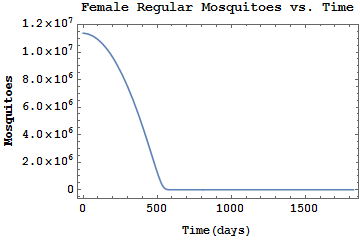
\includegraphics[width=\linewidth]{FrVst}
  \caption{$F_R$ vs. time}
  \label{fig:frvst}
\end{figure}

From figure 1, we can see clearly from the plot that the female regular mosquitoes started with $F_R(0)=11375000$ as an initial condition, then gradually decreasing as time progresses. This behavior is expected as the population of regular mosquitoes should go down and eventually tend to zero.\\
\begin{figure}[h!]
  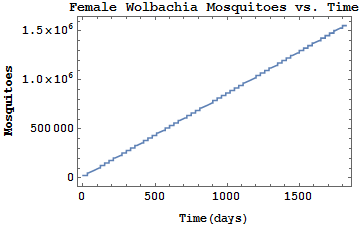
\includegraphics[width=\linewidth]{FwVSt}
  \caption{$F_W$ vs. time}
  \label{fig:fwvst}
\end{figure}

From figure 2, we can see the rise of the female \textit{Wolbachia}.  Again, this rise is as expected as each female \textit{Wolbachia} would be bear more offspring that can eventually take over the mosquitoes population. The step-like features are the effects of introducing new \textit{Wolbachia} mosquitoes to the population every month. \\

\begin{figure}[h!]
  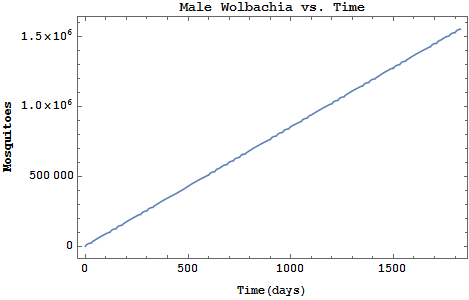
\includegraphics[width=\linewidth]{MwVsT}
  \caption{$M_W$ vs. time}
  \label{fig:mwvst}
\end{figure}

From figure 3, we can see that the population rises as expected and the tiny step-like features bear resemblance to that of the corresponding female curve. Again, such feature arises as we introduces more female mosquitoes that are capable of producing male and female offspring.\\

We decided not to plot $M_R$ since such population is of little interest to the problem. However, please note that we still account for their presence in the model for mating purposes.\\

\begin{figure}[h!]
  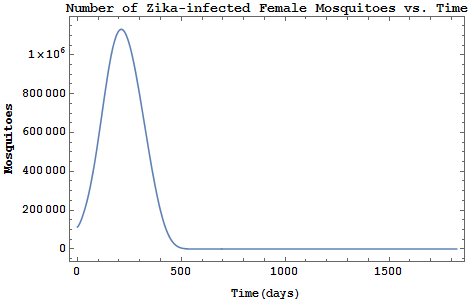
\includegraphics[width=\linewidth]{NzVSt}
  \caption{$N_z$ vs. time}
  \label{fig:nzvst}
\end{figure}

Furthermore, we can then model the population of Zika-infected Female as a function of time. Figure 4 shows the progression of this quantity. As expected, the number rises and peaks as the \textit{Wolbachia} is still taking time to dominate the mosquito population. However, as the \textit{Wolbachia} mosquitoes start to gain ground, the number of Zika-infected mosquitoes decline rapidly, tending to 0. Even at the peak of the Zika-infected mosquitoes, it is only 1 million - a small fraction of the total mosquito population considering that we initally started with 22 million total mosquitoes. \\

All these results confirm the expected behaviors of our model - demonstrating its validity. Furthermore, we can see clearly just how massive an impact of the female \textit{Wolbachia} mosquitoes have on the system of mosquitoes. Now, we can analyze the mosquitoes-human interaction, the main focus of our analysis.\\

\subsubsection{Human-Mosquito Dynamics}
\begin{figure}[h!]
  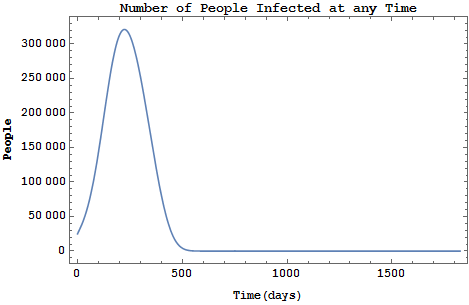
\includegraphics[width=\linewidth]{NhVSt}
  \caption{$N_h$ vs. time}
  \label{fig:nhvst}
\end{figure}
\begin{figure}[h!]
  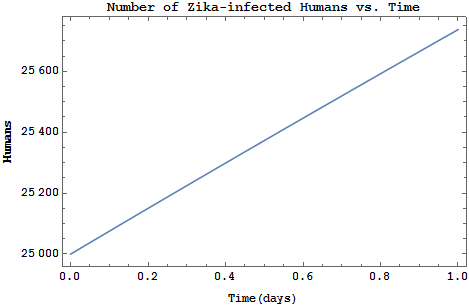
\includegraphics[width=\linewidth]{NhVst-init}
  \caption{$N_h$ vs. time (1 day span)}
  \label{fig:nhvstinit}
\end{figure}

Figure 5 and 6 shows the number of people infected with Zika at any time $t$. The advantage of having this knowledgeis the power to know exactly the percentage of population infected at any given time. From figure 4, we can see that the number of Zika-infected people rises, peak at around 365 days with more than 300,000 people infected, and declines tending to 0. Comparing figure 1, figure 4, and figure 5 will reveal that their rise and fall coincide significantly. This is reaffirming the validity of the model as the number of Zika-infected humans decrease as Zika-infected decreases and \textit{Wolbachia} mosquitoes increases.\\

Figure 6 shows the behavior of $N_h$ in a short time period of the first day. Examining figure 6 reveals that the slope $\frac{dN_h}{dt}\approx600$, affirming our initial condition that there is 600 infected case per day initially. \\

\begin{figure}[h!]
  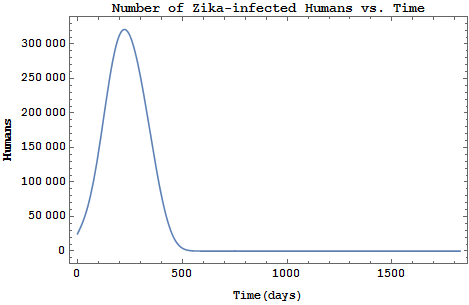
\includegraphics[width=\linewidth]{NzVst-Mw0=0}
  \caption{$N_z$ vs. time. $M_{W0}=0$}
  \label{fig:nzvstmw00}
\end{figure}

\begin{figure}[h!]
  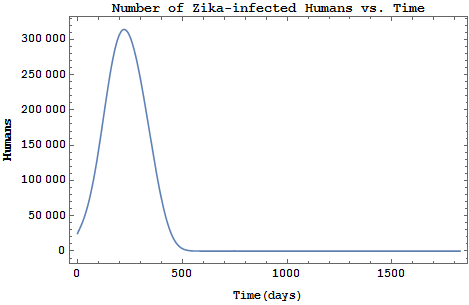
\includegraphics[width=\linewidth]{NzVst-Mw0=10000}
  \caption{$N_z$ vs. time. $M_{W0}=10000$}
  \label{fig:nzvstmw01000}
\end{figure}
Furthermore, in figures 7 and 8, we analyze if a change in $M_{W0}$ will create an impact on the system. Figure 7 is the number of Zika-infected humans if we introduce no male \textit{Wolbachia} every month, and figure 8 is if we introduce 10,000 male \textit{Wolbachia} every month. We can see that the difference is negligible and tiny. In fact, it's so similar in nature that it is almost-impossible to tell the difference even when putting them in close proximity. Thus, we concluded that introducing new male \textit{Wolbachia} every month is useless.
\subsubsection{Infections per Day}
As the number of new infections per day is an important criteria to limit, $\frac{dN_h}{dt}$ have been plotted over time in figure 9 to 11. \\
\begin{figure}[h!]
  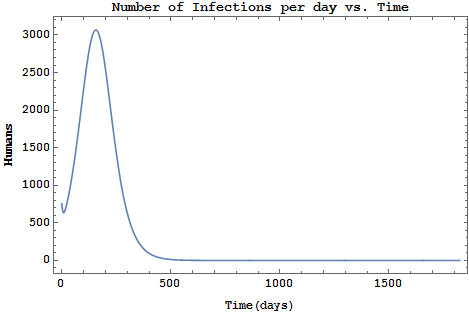
\includegraphics[width=\linewidth]{dNdtVst}
  \caption{$\frac{dN_h}{dt}$ vs. time}
  \label{fig:dndtvst}
\end{figure}

\begin{figure}[h!]
  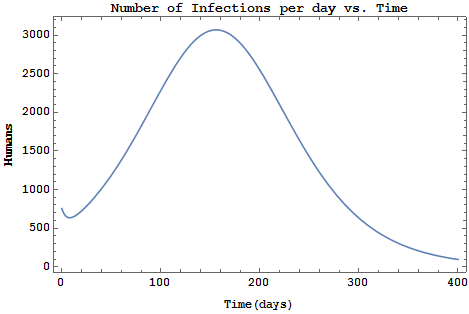
\includegraphics[width=\linewidth]{dNdtVst-tmax=400}
  \caption{$\frac{dN_h}{dt}$ vs. time}
  \label{fig:dndtvst400}
\end{figure}

\begin{figure}[h!]
  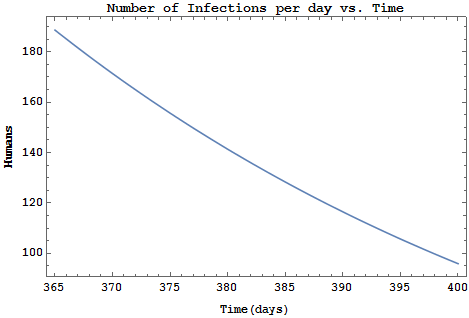
\includegraphics[width=\linewidth]{dNdtVst-tmin=365-tmax=400}
  \caption{$\frac{dN_h}{dt}$ vs. time}
  \label{fig:dndtvst400}
\end{figure}

\begin{figure}[h]
  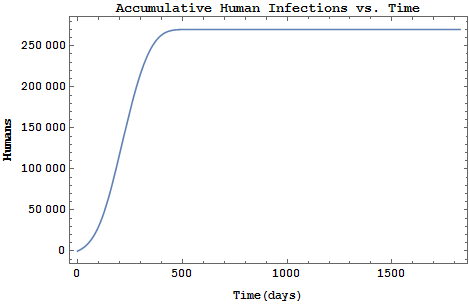
\includegraphics[width=\linewidth]{ntvst}
  \caption{$N_t$ vs. time}
  \label{fig:ntvst}
\end{figure}

\begin{figure}[h]
  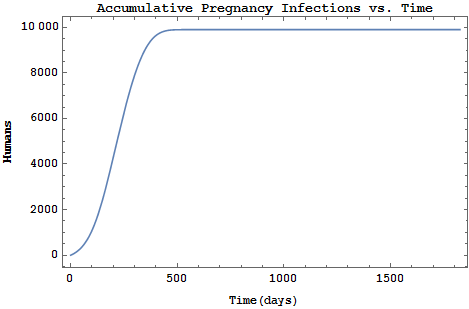
\includegraphics[width=\linewidth]{ntpregvst}
  \caption{$N_t$ of pregnant women vs. time}
  \label{fig:ntpregvst}
\end{figure}

Figure 9 shows the infection rate over the whole course of the program - 5 years. It is consequential that this figure 9 must closely resemble figure 5. Figure 10 shows that the infection rate does peak at around 190 days with a peak around 3000 infections per day. However, this is allowed since we only need to limit to be below 300 starting from the first year (day 365). Note that the plot of $\frac{dN_t}{dt}$ shows that $\frac{dN_t}{dt}>0$ for all time, meaning that the total population are still getting infected as time progresses - another reaffirmation. \textbf{Examining figure 11 reveals that starting from $t=365$, the infection rate is $\frac{dN_h}{dt}<200$ infections per day. Thus, our decision to use 25500 female and 0 male \textit{Wolbachia} does indeed satisfy the criteria of the prompt.}

\subsubsection{Total Humans Infected}

Evaluating equation (15) such that $N_t(1825)$ to find the total number of infected people in 5 years. We find that $N_t(1825)=270,025$ people if we introduce $F_{W0}=25500$ every month, as shown in figure 12.\\

Furthermore, we will assume that women pregnancy rate stays constant (based on the college student experience, we can say that the human coitus rate is fairly hard to change). The pregnancy rate is calculated to be $22/600\approx0.0366$. Using this, we can then model the number of infected pregnant women as shown in figure 13. \textbf{We calculated that exactly that $N_t(1825)=9901$. This number of total infected pregnant women is less than the total 10000 pregnant women, thus we meet the second criteria with 25500 female and 0 male \textit{Wolbachia}.}

\subsubsection{Process to Decision}

To reach a verdict of choosing 22,500 female and 0 male \textit{Wolbachia}, we first realized and evaluated the impact of the male \textit{Wolbachia} on the population as a whole. As it is bears negligible impact as explored earlier, we decided that it is in our best interest to not use them at all to reduce the total amount of mosquitoes released to nature - which the public will appreciate. Afterward, we use the \textbf{Manipulate} function in \textit{Mathematica} to evaluate manually which value of $F_{W0}$ would ensure that the total pregnancy not exceeding 10000. We then evaluate this value through $\frac{dN_h}{dt}$ to find out that with value we determined, the second criteria is still preserved. Thus, we decide on such value such that 25500 is the minimum amount of female \textit{Wolbachia} needed to be released to still satisfy the preconditions. We the found out that 25000 mosquitoes every month is not a large number of mosquitoes to be released since a city inf California - Clovis - has released 44000 \textit{Wolbachia} mosquitoes every week.

\section{Simulation Model}
We wrote a \textit{Java 8} program to model the mosquito population dynamics as \textit{Wolbachia} mosquitoes were released. The program models the male and female mosquito (extensions of the class mosquito). Mating is simulated using \textit{Java}'s random number generation function.\\

The code can be found in Appendix 2.\\

The results of our probabilistic program seemed to tally with our mathematical model.\\

How we developed the model:\\
We first wrote a representation of the mosquito. It had properties like age, lifespan and whether or not it carried \textit{Wolbachia}.\\

Then we extended this class to write representations of the male and the female mosquitoes, with their respective lifespans and susceptibility to infection. The females were given the ability to bite, mate, etc.\\

We wrote a class to represent humans. These humans had fell ill when bitten and got better in fourteen days. They could not develop immunity, but would not fall further ill on being bitten when already infected.\\

Finally, we tied things together with our main class.
The class prompts the user to provide initial population statistics. It initialises a number of mosquitoes and humans based on the set data.\\

It then follows the progress of time day-wise. Mosquitoes hatch, mate, age and bite. Humans get bitten, and get better. And so the quotidian processes continue in a virtual model for the number of months you want it to run. Every month the user gets an opportunity to release more \textit{Wolbachia} bearing mosquitoes.\\

The mating process that assigns a mate to a female uses pseudo random number generation to chose a random male from the adult male pool. Similarly, a pseudo random process determines which many humans are bitten.\\

Constants such as the rate of biting and transmission are taken as the same as in the mathematical model.\\

Differences in results may arise because of:\\
1. Random probabilistic process (simulation) as opposed to deterministic model (mathematical)\\
2. In the mathematical model, when mosquito population spikes, we take into consideration the fact that excessive competition for survival within the species will lead to a lower growth rate. We do not do this in the computer simulation.\\
3. The computer simulation accounts for delays due to growth. The mathematical model does not\\\\
The birth pattern of the female mosquito has been chosen to keep mosquito population stable had there been no \textit{Wolbachian} mosquitoes, because we do indeed believe that the mosquito population in nature is more or less stable.\\

The advantages of this model is that it is probabilistic, discrete and therefore closer to the real world. The chief disadvantage, unsurprisingly, arises from the same fact. The simulation can give us probable outcomes in various cases, but not reveal the actual dynamics behind the nature of a function. There are no graphs or reasoning; only some good estimates.\\

\section{Strengths and Weaknesses}
\subsection{Strengths}
The strongest asset of a model based on a purely mathematical framework is its universality of implementation. The basis of the framework lies correct if assumptions and logical advancements are made. We believe that employing a model such as one we developed will ensure accuracy in the long-term progression of the model due the flexibility of mathematics.\\

In addition, computation time is significantly reduced with a math-based model. Even for our model with at least 7 differential equations, \textit{Mathematica} is able to handle the implementation easily in less than one second. Comparing to the \textit{Java} simulation - through which we tested our model validity with a more probabilistic viewpoint, \textit{Mathematica} definitely and easily dominated the battle for time efficacy.\\

Furthermore, our model is deterministic: It is able to give accurate answer. Although this can also be a limitation due to the somewhat probabilistic, unpredictable nature of the world, it can also be an asset because it allows a deterministic solution from which we can extend a certain range in which the probability can fall. In other words, we have a good prediction of what nature should be.\\

It is also to note that if there are any changes are made to the constants or initial condition, we can easily implement those in matter of few keystrokes and new results in matter of minutes. As a result, we virtually have the model to handle all cases and extremities. From that, we can accurately model not only the Zika epidemic, but any other mosquito-vector based epidemic.\\
\subsection{Weaknesses}
The three greatest weakness of our model are:
\begin{enumerate}
    \item Lack of consideration for the incubation period of mosquitoes
    \item Lack of consideration for geographic and spatial density
    \item Lack of consideration for delay in birthrate, mortality rate, and all other rates
\end{enumerate}
Since the first weakness is fairly self-explanatory, we will expound on the latter two.\\

Any map of Puerto Rico population density shows that people are not evenly dispersed, and are heavily concentrated on the perimeter of the island. Furthermore, that density is non-linear in nature as urban center tends to disperse outward in a non-linearly deterministic manner. In addition, any existence of geographical boundaries will hinder the dispersal of mosquitoes. However, due the limited scope of our paper, we are unable to implement those. Finally, distance between places will also play a role in hindering mosquitoes transmission.\\

The delay in rates is another missing part of our work. This delay, although not significant and can corrected with $\epsilon$ as seen in Section 3, this delay in birthrate, deathrate, etc. will account for an even better model. Our current works on a long-term basis as in such a long span of time, our model acts as an average and this delay become negligible. However, if an accurate time-dependent depiction is necessary, delay is inevitable.\\


\section{Future Works}
Due to paucity of time, we were unable to work with equations that might take into consideration real world time-delay (since solving them would be harder). It would not be difficult to elaborate on our equations by adding temporal factors to take into account things like the exact number of people getting cured at a point of time, mosquito incubation period, etc. This would give take us closer to the real-world situation.\\
We would also be interested in getting better data for some constants that we had to indirectly calculate from other papers. It would be of considerable value to experimentally determine these constants. As a result, for future implementation, we require a system of delayed differential equations.\\

Geographical boundaries and limitations can be easily accounted for with a sufficient and extensive computer model working in conjunction with the mathematical model we developed. The only accurate way to depiction spread over real world data and boundaries can only be best represented through a computer simulation. This is the point where our computer simulation and mathematical model truly converge and work coherently for a better result. Due to the time limitation, we were only able to incorporate the computer simulation as a validation tool and a probabilistic affirmation of our mathematical model. If we want to incorporate geographical boundaries and spatial density, then truly both model and simulation can be unified coherently. Thus, another aspect for future improvement is the incorporation of spatial boundaries and features through both model and simulation.\\

\section{Conclusion}
In conclusion, we were able to develop a model based on a purely mathematical framework that encompasses immense flexibility and power of prediction. We also developed a simulation to work in conjunction to act as a probabilistic validation among many other validations mentioned in section 3. We tested many aspects of the model and they work in accordance to real-world expectations. Through the details expounded earlier in the paper, we can confidently claim that the model does indeed work as expected to model the real world. We then used this model to predict that will happen with a certain amount of female and male \textit{Wolbachia}. From such, we determined that a minimum of \textbf{25500 female \textit{Wolbachia} mosquitoes and 0 male} are required to be released every month, for 5 years. A detailed explanations have been presented in section 3. Therefore, our model fits realistic expectations and able to quickly find the minimum amount required. That being said, there are many things to be done as mentioned in section 7. Perhaps a better model improvement can be developed in the near future based on the theoretical framework we developed will be able to help governments and agencies around the world to eradicate the Zika epidemic and perhaps can even expanded to other mosquito-based epidemics.
\section{References}
\begin{enumerate}
    \item Beck-Johnson, Lindsay M., William A. Nelson, Krijn P. Paaijmans, Andrew F. Read, Matthew B. Thomas, and Ottar N. Bjørnstad. 2013. “The Effect of Temperature on Anopheles Mosquito Population Dynamics and the Potential for Malaria Transmission.”\\ PLoS ONE 8 (11). doi:10.1371/journal.pone.0079276.
    
    \item Center for Disease Control. n.d. “Dengue and the Aedes Aegypti Mosquito.” https://www.cdc.gov/dengue/resources/30Jan2012/aegyptifactsheet.pdf.
    
    \item ——. n.d. “Mosquito Life Cycle.”\\ http://www.cdc.gov/dengue/resources/factSheets/MosquitoLifecycleFINAL.pdf.
    
    \item Chaves, Luis F., Amy C. Morrison, Uriel D. Kitron, and Thomas W. Scott. 2011. “Nonlinear Impacts of Climatic Variability on the Density‐dependent Regulation of an Insect Vector of Disease.” ResearchGate 18 (2): 457–68. doi:10.1111/j.1365-2486.2011.02522.x.
    
    \item Couret, Jannelle, Ellen Dotson, and Mark Q. Benedict. 2014. “Temperature, Larval Diet, and Density Effects on Development Rate and Survival of Aedes Aegypti (Diptera: Culicidae).” PLoS ONE 9 (2).\\ doi:10.1371/journal.pone.0087468.
    
    \item “Does Zika Permanently Raise a Woman’s Pregnancy Risk?” 2016. STAT. April 19.\\ https://www.statnews.com/2016/04/19/zika-women-future-pregnancies/.
    
    \item Lloyd, Alun. n.d. “Mosquit-Borne Diseases: Modeling and Control.” http://www.theory.physics.manchester.ac.uk/complexitymeeting/lloyd.pdf.
    
    \item Lounibos, L. Philip, and Richard L. Escher. 2008. “SEX RATIOS OF MOSQUITOES FROM LONG-TERM CENSUSES OF FLORIDA TREE HOLES.” Journal of the American Mosquito Control Association 24 (1): 11–15.
    
    \item Mayer, M.S. 1966. “Decline in Male/Female Sex Ratio of Aedes Aegypti (L.) During Hatching.” JAMCA, March.
    
    \item Morin, Cory, Andrew Comrie, and Ermst Kacey. 2016. “EHP – Climate and Dengue Transmission: Evidence and Implications.” Accessed November 21. http://ehp.niehs.nih.gov/1306556/.
    
    \item “Mosquitoes and Disease.” 2016. Accessed November 21.\\ http://www.idph.state.il.us/envhealth/pcmosquitoes.htm.
    
    \item Society, National Geographic. 2016. “Mosquitoes, Mosquito Pictures,\\ Mosquito Facts - National Geographic.” \\Accessed November 20. \\http://animals.nationalgeographic.com/animals/bugs/mosquito/.
    
    \item Team, National Weather Service Corporate Image Web. \\
    2016. “National Weather Service Climate.” \\Accessed November 21.\\ \verb!http://w2.weather.gov/climate/local_data.php?wfo=sju!.
    
    \item Thangamani, Saravanan, Jing Huang, Charles E. Hart, Hilda Guzman, and Robert B. Tesh. 2016. “Vertical Transmission of Zika Virus in Aedes Aegypti Mosquitoes.” The American Journal of Tropical Medicine and Hygiene 95 (5): 1169–73. doi:10.4269/ajtmh.16-0448.
    
    \item U.S. Census. n.d. “U.S. Government Census: Puerto Rico 2010.”\\ https://www.census.gov/prod/cen2010/cph-1-53.pdf.
    
    \item Zheng, Bo, Moxun Tang, and Jianshe Yu. 2014. “Modeling Wolbachia Spread in Mosquitoes Through Delay Differential Equations.” SIAM Journal on Applied Mathematics 74 (3): 743–70.\\ doi:http://dx.doi.org/10.1137/13093354X.
    
    \item “Zika Virus.” 2014. CDC. November 5.\\ http://www.cdc.gov/zika/vector/range.html. 
\end{enumerate}
    


\section{Appendix 1 \textit{Mathematica} Math Model}
Due to the incredibly challenging nature to put \textit{Mathematica} code in Latex, we have included a picture (figure 14) for easier reading and reference. Please go to our git repository to get the \textit{Mathematica} notebook: https://github.com/iarbak/zika
\begin{figure}[H]
  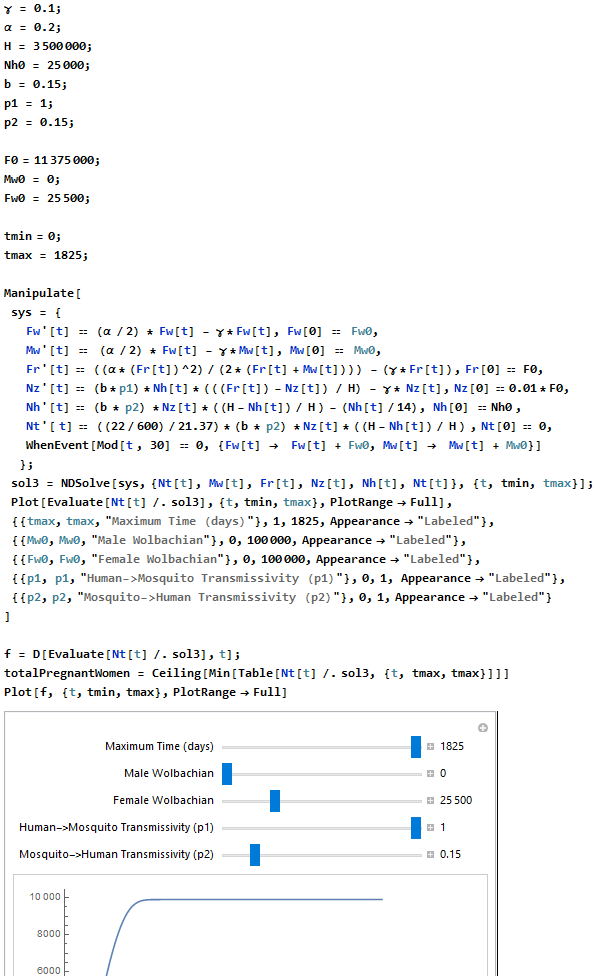
\includegraphics[width=\linewidth]{mathematica}
  \caption{Mathematica Implementation}
  \label{fig:math}
\end{figure}
\section{Appendix 2 \textit{Java} Simulation}
Please use the source code from our git repository at: https://github.com/iarbak/zika. This will ensure better quality of code readability.\\
The code below are left for reference, we do not recommend reading from this since LaTeX does not format codes very nicely.

\subsection{Class Mosquito}
\lstset{language=Java}
\begin{lstlisting}[frame=None]
package model;

/**
 * This class models the generic mosquito and must be extended
 * 
 * @author aditi
 *
 */
public abstract class Mosquito {

	public int age;
	int lifeSpan;
	boolean infected;
	// does this mosquito carry Zika?

	enum type {
		W, R
	}; // wolbachian and regular

	public boolean alive; // is the mosquito alive?
	public boolean adult; // is it capable of reproduction?
	type T; // store type of mosquito

	/**
	 * Constructor t is 0 if wolbachian, 1 if not
	 */
	Mosquito(int t) {
		age = 0;
		alive = true;
		adult = false;
		genLifespan();
		infected = false;
		setType(t);
	}

	/**
	 * id this mosquito an adult
	 */
	public boolean isAdult() {
		return adult && alive;
	}

	/**
	 * returns type in integer
	 * 
	 * @return
	 */
	public int getType() {
		return T.ordinal();
	}

	/**
	 * constructor that intiialises for a specific age
	 * 
	 * @param t=mosquito
	 *            type: 0 for wolbachian, 1 for regular
	 * @param age
	 *            =age in days
	 */
	Mosquito(int t, int age) {
		this(t);
		this.age = age;
	}

	/**
	 * sets whether Wolbachian or not. 0 is Wolbachian 1 is regular.
	 * 
	 * @param t
	 */
	void setType(int t) {
		switch (t) {
		case 0:
			T = type.W;
			break;
		case 1:
			T = type.R;
		}
	}

	/**
	 * Generates lifespan based on mosquito gender and assigns it to variable
	 * lifespan
	 */
	void genLifespan() {
	};

	/**
	 * changes variables with progress of a day
	 */
	public void update() {
		age++;
		if (age >= 15)
			adult = true;
		if (age > lifeSpan) {
			alive = false;
			adult = false;
		}
	}
}
\end{lstlisting}
\subsection{Female mosquito}
\begin{lstlisting}[frame=None]
package model;

/**
 * This class models the female mosquito
 */
public class Female extends Mosquito {

	boolean fertile = false;
	// depending on mate, can female produce offspring
	type child;
	// if so, what kind of offspring (W or regular)?

	/**
	 * constructor t= 0 for Wolbachian, 1 for regular
	 * 
	 * @param t
	 */
	public Female(int t) {
		super(t);
	}

	public Female(int t, int age) {
		super(t, age);
	}

	/**
	 * method to construct possibly zika infected mosquito
	 * 
	 * @param t
	 * @param infected
	 */
	public Female(int t, boolean infected) {
		this(t);
		if (t == 1) {
			this.infected = infected;
		}
	}

	/**
	 * method to construct possibly infected female
	 * 
	 * @param t
	 *            is the type of mosquito
	 * @param age
	 *            is age of the mosquito
	 * @param infected
	 *            is whether the mosquito received the virus
	 */
	public Female(int t, int age, boolean infected) {
		this(t, age);
		if (t == 1) {
			this.infected = infected;
		}
	}

	/**
	 * How does biting a human affect the mosquito
	 * 
	 * @param h
	 */
	public void bite(Human h) {
		if (h.infected)
			if (T == type.R)
				infected = true;
	}

	@Override
	void genLifespan() {
		lifeSpan = 55; // 40 days adult
	}

	/**
	 * returns child type
	 * 
	 * @return
	 */
	public int childType() {
		return child.ordinal();
	}

	/**
	 * determines offspring type depending on mate m
	 * 
	 * @param m
	 */
	public void mate(Male m) {
		if (this.T == type.R) {
			if (m.T == type.R) {
				fertile = true;
				child = type.R;
			} else {
				fertile = false;
				child = null;
			}
		} else {
			fertile = true;
			child = type.W;
		}
	}

	/**
	 * returns value of fertile
	 */
	public boolean isFertile() {
		return fertile;
	}

	/**
	 * Will the mosquito produce a child today? 0 if no. 1 if male 2 if female
	 * 
	 * @return
	 */
	public int produceChild() {
		if (fertile) {
			if (age == 35) {
				return 2;
			} else if (age == 15 || age == 25 || age == 45 || age == 55)
				return 1;
		}
		return 0;
	}
}
\end{lstlisting}
\subsection{Male mosquito}
\begin{lstlisting}
package model;

/**
 * This class is a model of the male mosquito
 * 
 * @author aditi
 *
 */
public class Male extends Mosquito {

	/**
	 * constructor t= 0 for Wolbachian, 1 for regular
	 * 
	 * @param t
	 */
	public Male(int t) {
		super(t);
	}

	public Male(int t, int age) {
		super(t, age);
	}

	@Override
	void genLifespan() {
		lifeSpan = 25; // 10 days as adult, 15 as egg/larva
	}
}
\end{lstlisting}
\subsection{Human}
\begin{lstlisting}
package model;

public class Human {

	public boolean infected;
	public boolean pregnant;
	int daySince; // day since the human was bitten

	/**
	 * default constructor
	 */
	public Human(boolean infect) {
		infected = infect;
		pregnant = false;
		daySince = 15;
	}

	/**
	 * parametrized constructor: p is whether this human is pregnant
	 */
	public Human(boolean infect, boolean p) {
		this(infect);
		pregnant = p;
	}

	/**
	 * What happens to the human if it is bitten
	 * 
	 * @param m
	 *            is the mosquito that bites
	 */
	public void bitten(Mosquito m) {
		if (m.infected && !infected) {
			double random = (Math.random()); // transmission chance is half
			if (random < 0.5) {
				infected = true;
				daySince = 0;
			}
		}
	}

	public void update() {
		if (daySince < Integer.MAX_VALUE)
			daySince++;
		else
			daySince = 15;
		if (daySince > 14)
			infected = false;
	}
}
\end{lstlisting}

\subsection{Main simulation}
\begin{lstlisting}
package controller;

import java.lang.reflect.Field;
import java.util.ArrayList;
import java.util.HashMap;
import java.util.Iterator;
import java.util.List;
import java.util.Map.Entry;
import java.util.Random;
import java.util.Scanner;
import java.util.concurrent.ConcurrentHashMap;

import model.Female;
import model.Human;
import model.Male;

/**
 * runs the actual simulation
 * 
 * @author aditi some assumptions: 1. female mosquito only mates once (based on
 *         actual mosquito behaviour 2. female mosquito produces one female
 *         mosquito at 20th day of adult phase and 4 males at 0, 10, 30 and 40th
 *         day. This has been assumed to keep population stable and gender ratio
 *         well distributed as 1:1
 */
public class Main {
	static Scanner sc = new Scanner(System.in);

	static ConcurrentHashMap<Female, Integer> f = new ConcurrentHashMap(10000000);

	static ConcurrentHashMap<Male, Integer> m = new ConcurrentHashMap(10000000);
	static Field table = null;

	static {
		try {
			table = HashMap.class.getDeclaredField("table");
		} catch (NoSuchFieldException e) {
			// TODO Auto-generated catch block
			e.printStackTrace();
		} catch (SecurityException e) {
			// TODO Auto-generated catch block
			e.printStackTrace();
		}
		table.setAccessible(true);
	}

	static HashMap<Human, Integer> h = new HashMap(1000000);
	static int day = 0; // day number in simulation
	// population of mosquitos:
	static int fr, mr, fw, mw;
	static int totMonths;
	static int month = 0;
	static int pop; // population: number of humans
	static int totpreg = 0; // total pregnant women

	static Random r = new Random();

	public static void main(String[] args) {
		init();
		// females that ought to mate
		HashMap<Female, Integer> mateablef = new HashMap(1000);
		// males that ought to mate
		HashMap<Male, Integer> mateablem = new HashMap(1000);
		for (Female F : f.keySet()) {
			if (F.age == 15)
				mateablef.put(F, 0);
		}
		for (Male M : m.keySet()) {
			if (M.age == 15 && M.alive)
				mateablem.put(M, 0);
		}
		mate(mateablef, mateablem);
		mateablef.clear();
		mateablem.clear();

		while (month < totMonths) {
			if (month != 0)
				wulbach(month);
			// 30 days to the month

			for (int day = 0; day < 30; day++) {
				// first all the mosquito spawning

				for (Female F : f.keySet()) {
					switch (F.produceChild()) {
					case 0:
						break;
					case 1:
						m.put(new Male(F.childType(), 0), 0);
						break;
					case 2:
						f.put(new Female(F.childType(), 0), 0);
					}
				}
				// mating again
				for (Female F : f.keySet()) {
					if (F.age == 15)
						mateablef.put(F, 0);
				}
				for (Male M : m.keySet()) {
					if (M.age >= 15)
						mateablem.put(M, 0);
				}
				mate(mateablef, mateablem);
				mateablef.clear();
				mateablem.clear();
				// now all our mosquitoes age, we weed out the dead

				for (Female F : f.keySet()) {
					F.update();
					if (!F.alive)
						f.remove(F);
				}

				for (Male M : m.keySet()) {
					M.update();
					if (!M.alive)
						m.remove(M);
				}

				// humans progressing on the path to recovery
				for (Human H : h.keySet()) {
					H.update();
				}
				// mosquitoes bite
				bite(f, h);

				// end of day

				if (day % 5 == 0) {
					print(f, m);
				}
			}
			month++;
		}
		System.out.println("Total number of pregnant women afftected: " + totpreg);
	}

	/**
	 * Simulates mating of input female list with current adult males randomly
	 * we assume in this simulation that a female only mates once
	 */
	static void mate(HashMap<Female, Integer> mateableF, HashMap<Male, Integer> mateablem) {
		for (Female F : mateableF.keySet()) {
			// generate random index of male to mate with
			Male M = (Male) randomKey(mateablem);
			F.mate(M);
		}
	}

	/**
	 * Accepts initial conditions from users, initialises mosquito population
	 * with random ages
	 */
	static void init() {
		// initialising human population
		System.out.println("Enter number of humans:");
		pop = sc.nextInt();
		int infec = (int) ((double) pop * 0.07);
		for (int i = 0; i < pop; i++) {
			boolean infected = i % infec == 0;
			if (i % 30 == 0) // 0.033 is taken as % of humans pregnant
				h.put(new Human(infected, true), 0);
			else
				h.put(new Human(infected), 0);
		}

		// initialising previously present mosquito population
		System.out.println("Enter orignal regular female population:");
		fr = sc.nextInt();
		System.out.println("Enter original regular male population:");
		mr = sc.nextInt();
		wulbach(0);
		System.out.println("Enter number of months the simulation should run:");
		totMonths = sc.nextInt();
		for (int i = 0; i < fr; i++) {
			int age = r.nextInt(41) + 15;
			if (i % 50 == 0 && i % 100 != 0) // 1% population infected
				f.put(new Female(1, age, true), 0);
			else
				f.put(new Female(1, age), 0);
		}
		for (int i = 0; i < mr; i++) {
			int age = r.nextInt(41) + 15;
			m.put(new Male(1, age), 0);
		}
	}

	/**
	 * Handles biting event
	 * 
	 * @param h
	 *            human who is bitten
	 * @param f
	 *            mosquito that bites the human
	 */
	static void handleBite(Human h, Female f) {
		f.bite(h);
		if (!h.infected) {
			h.bitten(f);
			if (h.infected && h.pregnant)
				totpreg++;
		}
	}

	/**
	 * Mosquitoes in f bite humans in h
	 * 
	 * @param f2
	 * @param m
	 */
	static void bite(ConcurrentHashMap<Female, Integer> f2, HashMap<Human, Integer> h) {
		if (h.size() > 0) {
			for (Female F : f2.keySet()) {
				// bite rate is 0.15
				if (r.nextDouble() < 0.15) {
					// generate random index of human to bite

					// int index = (h.size() == 0) ? 0 : r.nextInt(h.size());
					// List<Human> keys = new ArrayList<Human>(h.keySet());

					Human H = (Human) randomKey(h);
					handleBite(H, F);
				}
			}
		}
	}

	/**
	 * input wolbachians you are releasing i is month number assume all adults
	 * are newly hatched
	 * 
	 * @param i
	 */
	static void wulbach(int j) {
		System.out.println("Enter wolbachian female population released in month " + j + ":");
		fw = sc.nextInt();
		System.out.println("Enter wolbachian male population released in month " + j + ":");
		mw = sc.nextInt();
		for (int i = 0; i < fw; i++) {
			f.put(new Female(0, 15), 0);
		}
		for (int i = 0; i < mw; i++)
			m.put(new Male(0, 15), 0);
	}

	/**
	 * prints population statistics
	 * 
	 * @param f2
	 *            array of females
	 * @param m2
	 *            array of males
	 */
	static void print(ConcurrentHashMap<Female, Integer> f2, ConcurrentHashMap<Male, Integer> m2) {
		int count = 0;
		for (Female F : f2.keySet()) {
			if (F.getType() == 0)
				count++;
		}
		System.out.println("Number of female Wulbachians: " + count);
		System.out.println("Number of female Regular: " + (f2.size() - count));
		count = 0;
		for (Male M : m2.keySet()) {
			if (M.getType() == 0)
				count++;
		}
		System.out.println("Number of male Wulbachians: " + count);
		System.out.println("Number of male Regular: " + (m2.size() - count));

		count = 0;
		int p = 0;
		for (Human H : h.keySet()) {
			if (H.infected) {
				count++;
				if (H.pregnant)
					p++;
			}
		}
		System.out.println("Number of humans infected: " + count);
		System.out.println("Number of them that are pregnant: " + p);
		System.out.println();
	}

	public static Object randomKey(HashMap map) {
		Entry[] entries = null;
		try {
			entries = (Entry[]) table.get(map);
		} catch (IllegalArgumentException | IllegalAccessException e) {
			// TODO Auto-generated catch block
			e.printStackTrace();
		}
		int start = r.nextInt(entries.length);
		for (int i = 0; i < entries.length; i++) {
			int idx = (start + i) % entries.length;
			Entry entry = entries[idx];
			if (entry != null)
				return entry.getKey();
		}
		return null;
	}

}

\end{lstlisting}

\end{document}
